%%
%% This is file `sample-xelatex.tex',
%% generated with the docstrip utility.
%%
%% The original source files were:
%%
%% samples.dtx  (with options: `sigconf')
%% 
%% IMPORTANT NOTICE:
%% 
%% For the copyright see the source file.
%% 
%% Any modified versions of this file must be renamed
%% with new filenames distinct from sample-xelatex.tex.
%% 
%% For distribution of the original source see the terms
%% for copying and modification in the file samples.dtx.
%% 
%% This generated file may be distributed as long as the
%% original source files, as listed above, are part of the
%% same distribution. (The sources need not necessarily be
%% in the same archive or directory.)
%%

\documentclass[sigconf, nonacm]{acmart}

\usepackage{mwe}
\usepackage[colorinlistoftodos,prependcaption,textsize=tiny]{todonotes}
\usepackage{cleveref}

%%
%% \BibTeX command to typeset BibTeX logo in the docs
\AtBeginDocument{%
  \providecommand\BibTeX{{%
    \normalfont B\kern-0.5em{\scshape i\kern-0.25em b}\kern-0.8em\TeX}}}

\begin{document}

%%
%% The "title" command has an optional parameter,
%% allowing the author to define a "short title" to be used in page headers.
\title{Bringing Packet Queueing to XDP}

%%
%% The "author" command and its associated commands are used to define
%% the authors and their affiliations.
%% Of note is the shared affiliation of the first two authors, and the
%% "authornote" and "authornotemark" commands
%% used to denote shared contribution to the research.
\author{Freysteinn Alfreðsson}
\email{freysteinn.alfredsson@kau.se}
\orcid{0000-0003-1516-9370}
\affiliation{%
  \institution{Department of Computer Science}
  \city{Karlstad}
  \country{Sweden}
}
\author{Per Hurtig}
\email{per.hurtig@kau.se}
\affiliation{%
  \institution{Department of Computer Science}
  \city{Karlstad}
  \country{Sweden}
}
%%\orcid{0000-0003-1516-9370}
\author{Anna Brunstrom}
\email{anna.brunstrom@kau.se}
\affiliation{%
  \institution{Department of Computer Science}
  \city{Karlstad}
  \country{Sweden}
}

\author{Toke Høiland-Jørgensen}
\email{toke@redhat.com}
\affiliation{%
  \institution{Red hat}
  \country{Denmark}
}

\author{Jesper Dangaard Brouer}
\email{brouer@redhat.com}
\affiliation{%
  \institution{Red hat}
  \country{Denmark}
}

%%
%% By default, the full list of authors will be used in the page
%% headers. Often, this list is too long, and will overlap
%% other information printed in the page headers. This command allows
%% the author to define a more concise list
%% of authors' names for this purpose.
\renewcommand{\shortauthors}{Alfreðsson, et al.}

\begin{abstract}

The Linux eXpress Data Path, or XDP, has found numerous uses in the industry, such as DoS attack mitigation, load-balancers, and intrusion prevention systems. XDP provides a high-performance programmable network data path using the BPF framework and allows programmers to process packets early out of the driver. While XDP excels in forwarding packets, it currently has no mechanism for queueing or reordering packets and cannot implement traffic scheduling policies. In this paper, we present our ongoing work to address this challenge. We have designed a programmable packet scheduling extension for the XDP framework using recently proposed schemes for programmable queues. This extension allows programmers to define their packet schedulers using BPF while benefiting from the XDP fast data path.

\end{abstract}

%%
%% Keywords. The author(s) should pick words that accurately describe
%% the work being presented. Separate the keywords with commas.
\keywords{XDP, BPF, eBPF, Queueing, Linux, Scheduling, Programmable scheduling}

%%
%% This command processes the author and affiliation and title
%% information and builds the first part of the formatted document.
\maketitle

\section{Introduction}

The Linux kernel is a widely used platform in devices that range from IoT, cellphones, home and enterprise routers to servers and cloud offerings. One of the prominent technologies of the Linux kernel is the BPF~\footnote{TODO} framework~\cite{ebpf}, which gives us a flexible way to extend the kernel. The BPF framework is an in-kernel runtime environment that allows domain-specific code to execute within the kernel safely using predefined hooks. One such hook is the Linux eXpress Data Pat~\cite{hoiland2018express}, or XDP, which introduces a fast data-path within the Linux kernel and has found numerous uses in the industry such as Denial-of-Service~\cite{bertin2017xdp}~\cite{miano2019introducing} (DoS) attack-mitigation, load-balancers, and intrusion prevention systems.

XDP provides a high-performance programmable network data path and allows programmers to process packets early out of the driver and even bypass the kernel's network stack for increased performance. While XDP excels in forwarding packets, it currently has no mechanism for queuing or reordering packets and can not implement traffic scheduling policies. Packet scheduling is a common task on network equipment, and most devices that provide packet scheduling algorithms provide only a handful of predefined packet schedulers. The Linux kernel's network stack provides a traffic control system called Queuing discipline (Qdisc) capable of packet scheduling. However, it does not provide the means of implementing complete packet schedulers in BPF, nor can it be used in XDP when bypassing the kernel's networking stack. Therefore, a new extension to XDP is needed.

This paper presents our work on adding programmable packet scheduling to XDP. We have designed a programmable packet scheduling framework in BPF using recently proposed schemes for programmable queues. This extension allows programmers to define their packet schedulers using BPF while benefiting from the XDP fast data path.

The rest of the paper is structured as follows: (i) we present a short overview of what packet schedulers are; (ii) an overview of the Linux kernel's networking subsystems and why there is an interest in bypassing it; (iii) what programmable packet schedulers are; (iv) how the PIFO provides us with a fast and generalized data structure to express most schedulers; (v) a short overview of the BPF framework and XDP; (vi) our contribution, a programmable packet scheduling framework in BPF; (vii) future work; (viii) and finally, our conclusion.


% Frey: The last paragraph could be rewritten to list the contributions.
% - A BPF packet scheduling framework.
% - XDP with queueing using the new framework.
% - Qdisc with queueing using the new framework.
% - Evaluation of the new framework.


\section{Packet Scheduling, Traffic Shaping, and Queue Management}

Packet schedulers provide the means of controlling the policy and quality requirements within a network for customers and services. However, at its core, the primary function of the packet scheduler is to arrange or rearrange packets to meet the requirements of the network. Most of these requirements improve the latency of specific flows or improve fairness between flows. For instance, video streaming services would like to ensure that clients get fair access to their video streams. Moreover, a service provider might want to prioritize traffic of their production servers over their testing servers. Therefore, having the flexibility to adapt the packet scheduling algorithm to the requirements of the network in question can significantly improve its overall quality.

\begin{figure}
  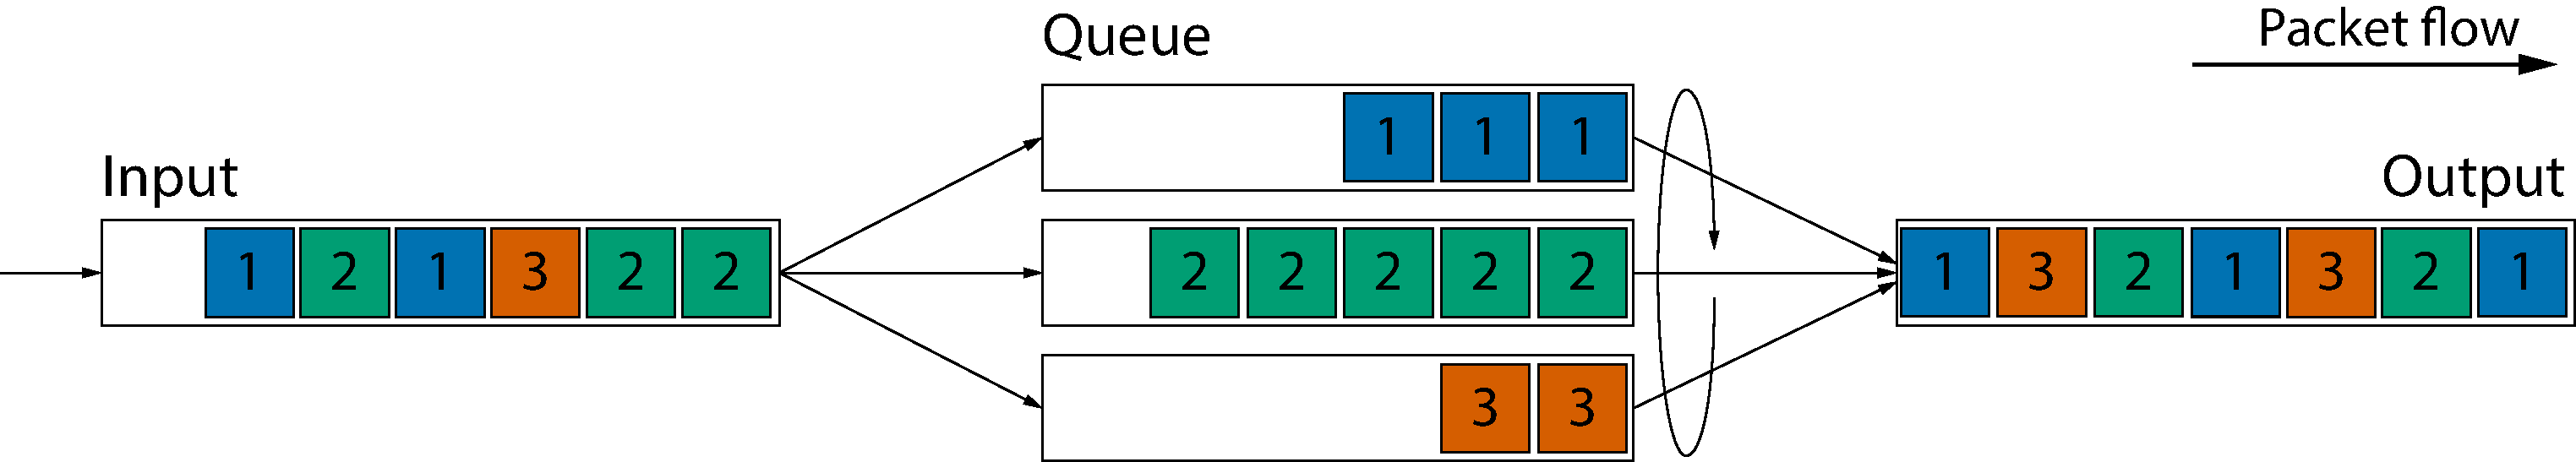
\includegraphics[width=\linewidth]{round-robin.pdf}
  \caption{The Round-Robin scheduler sorts enqueued packets into different queues depending on their flows. On dequeue, the packets are dequeued in a round-robin fashion, giving equal throughput for flows when all packets are equal in size.}
  \label{fig:round_robin}
\end{figure}

For example, if we wanted to give equal throughput to three different clients that have equal size packets, we could use the round-robin scheduler~\cite{nagle1987packet}, depicted in \Cref{fig:round_robin}. This scheduler sorts the incoming packets by flow into different queues and dequeues the packets by taking one packet from each flow.

%\begin{figure}
%  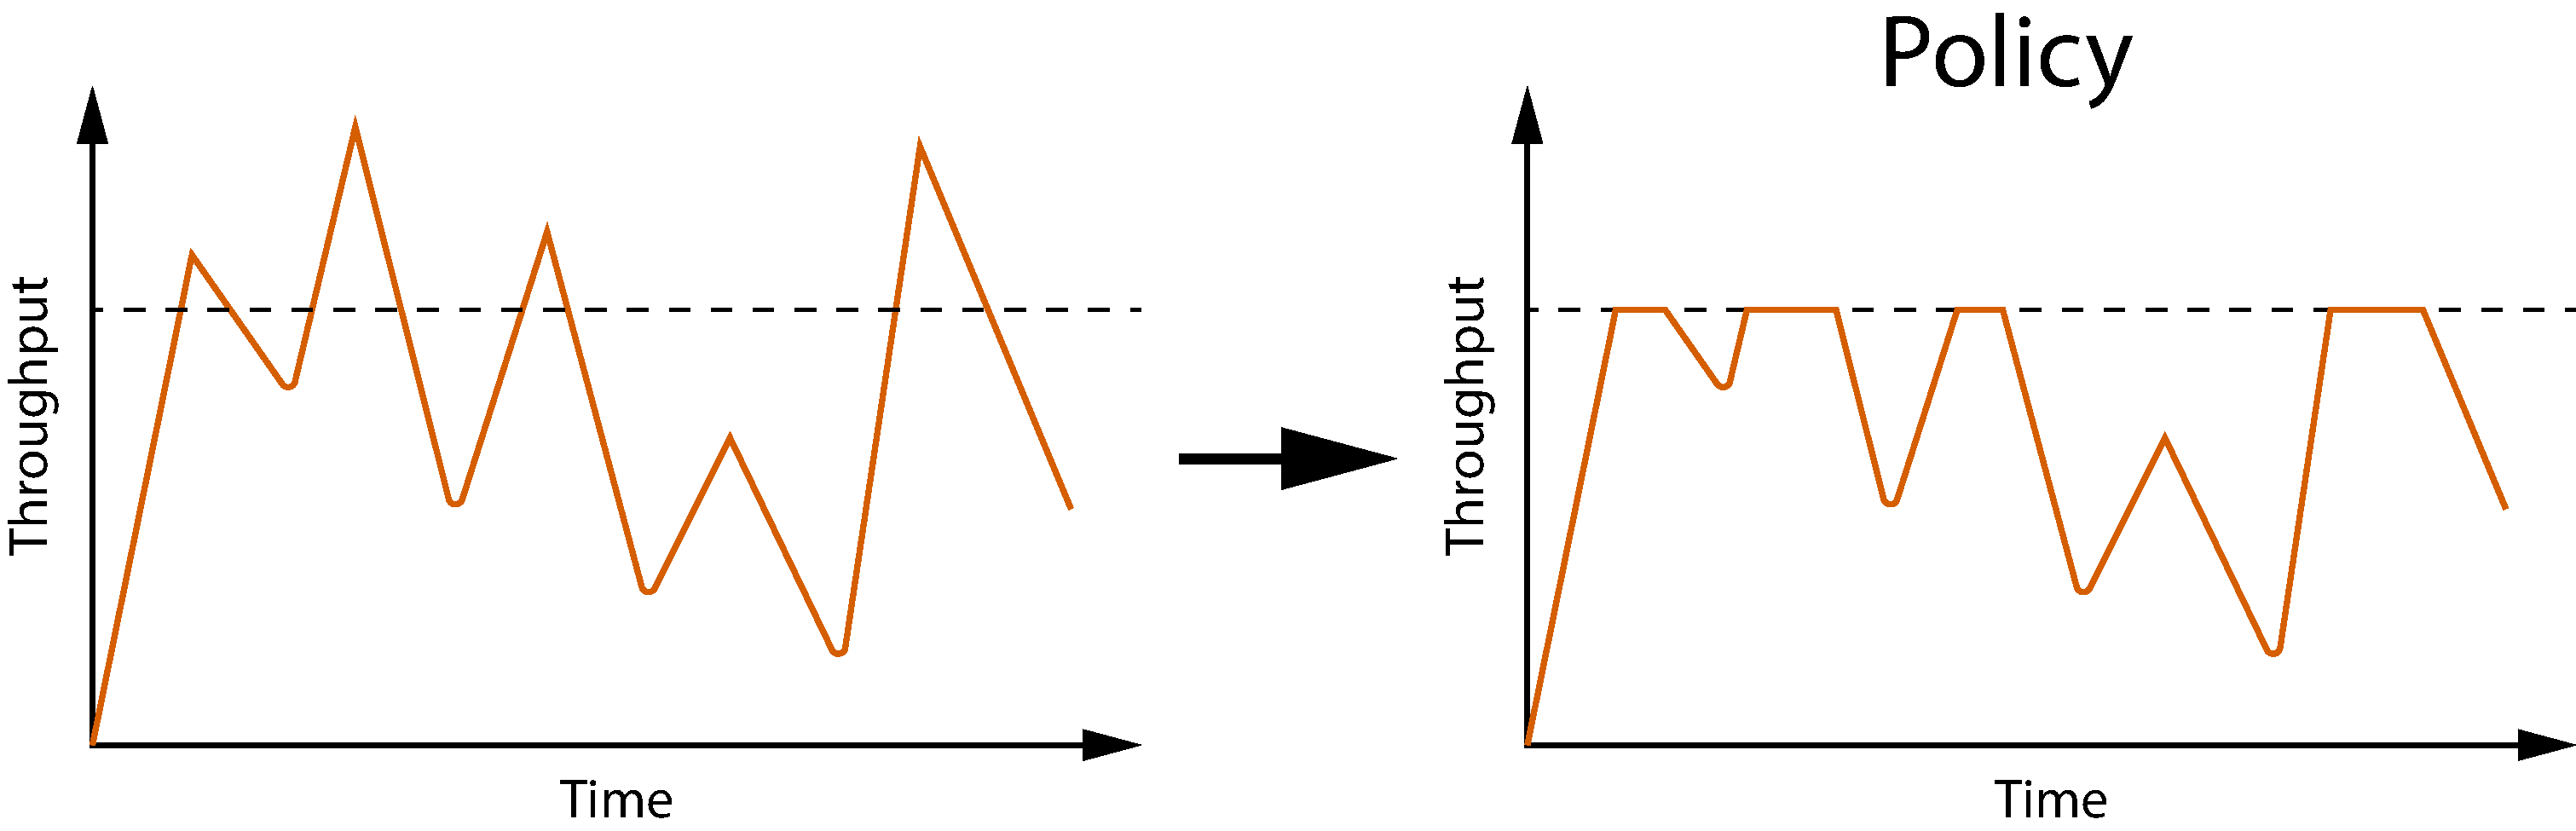
\includegraphics[width=\linewidth]{traffic-policy.pdf}
%  \caption{\label{fig:traffic_policy}}
%\end{figure}

\begin{figure}
  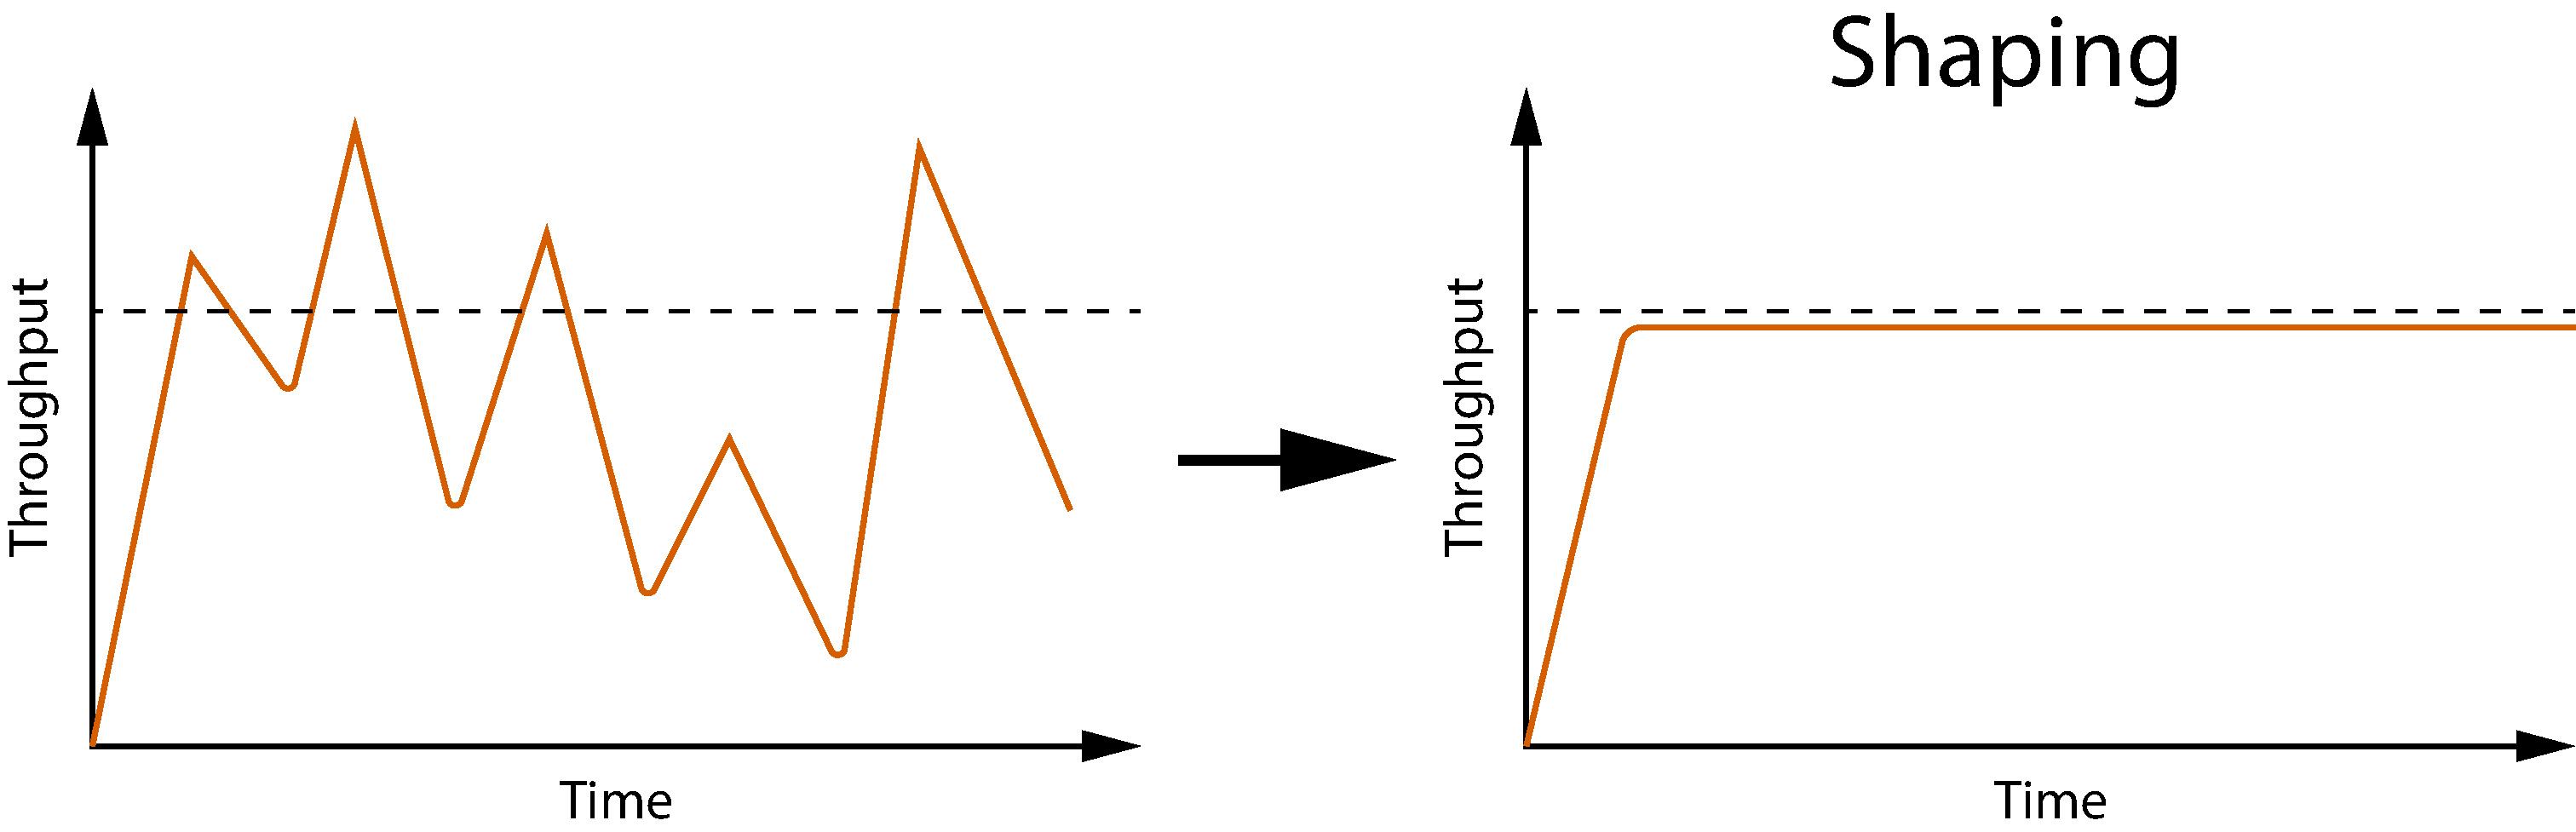
\includegraphics[width=\linewidth]{traffic-shaping.pdf}
  \caption{Traffic shaping is the art of delaying packets to control the throughput. The figure depicts traffic without shaping on the left and the same traffic with shaping on the right.}
  \label{fig:traffic_shaping}
\end{figure}

Another crucial component related to packet scheduling is the capability of delaying packets. This capability allows packet scheduling algorithms to provide traffic shaping, as seen in \Cref{fig:traffic_shaping}. Shaping algorithms are referred to as non-work conserving algorithms because they do not necessarily use the total capacity of the network interface, while work-conserving algorithms never delay packets and can use their total capacity. An example of a non-work conserving scheduling algorithm would be an ISP enforcing a network policy that guarantees their clients a certain bandwidth.

Queue management is also an essential topic related to packet scheduling and is the art of controlling how many packets that can be queued. A significant problem in today's environments is bufferbloat~\cite{gettys2011bufferbloat}, where network vendors have previously favored large buffers for throughput by sacrificing latency. Bufferbloat~\cite{TODO} can negatively affect low latency applications such as video conferencing, online gaming, and other interactive applications. Therefore, queue management is an integral part of the queueing process while not usually considered part of the packet scheduling algorithm.

% Frey: This last paragraph should contain a bit more about what bufferbloat is.

\section{The Linux Kernel Networking Subsystem}

\begin{figure}
  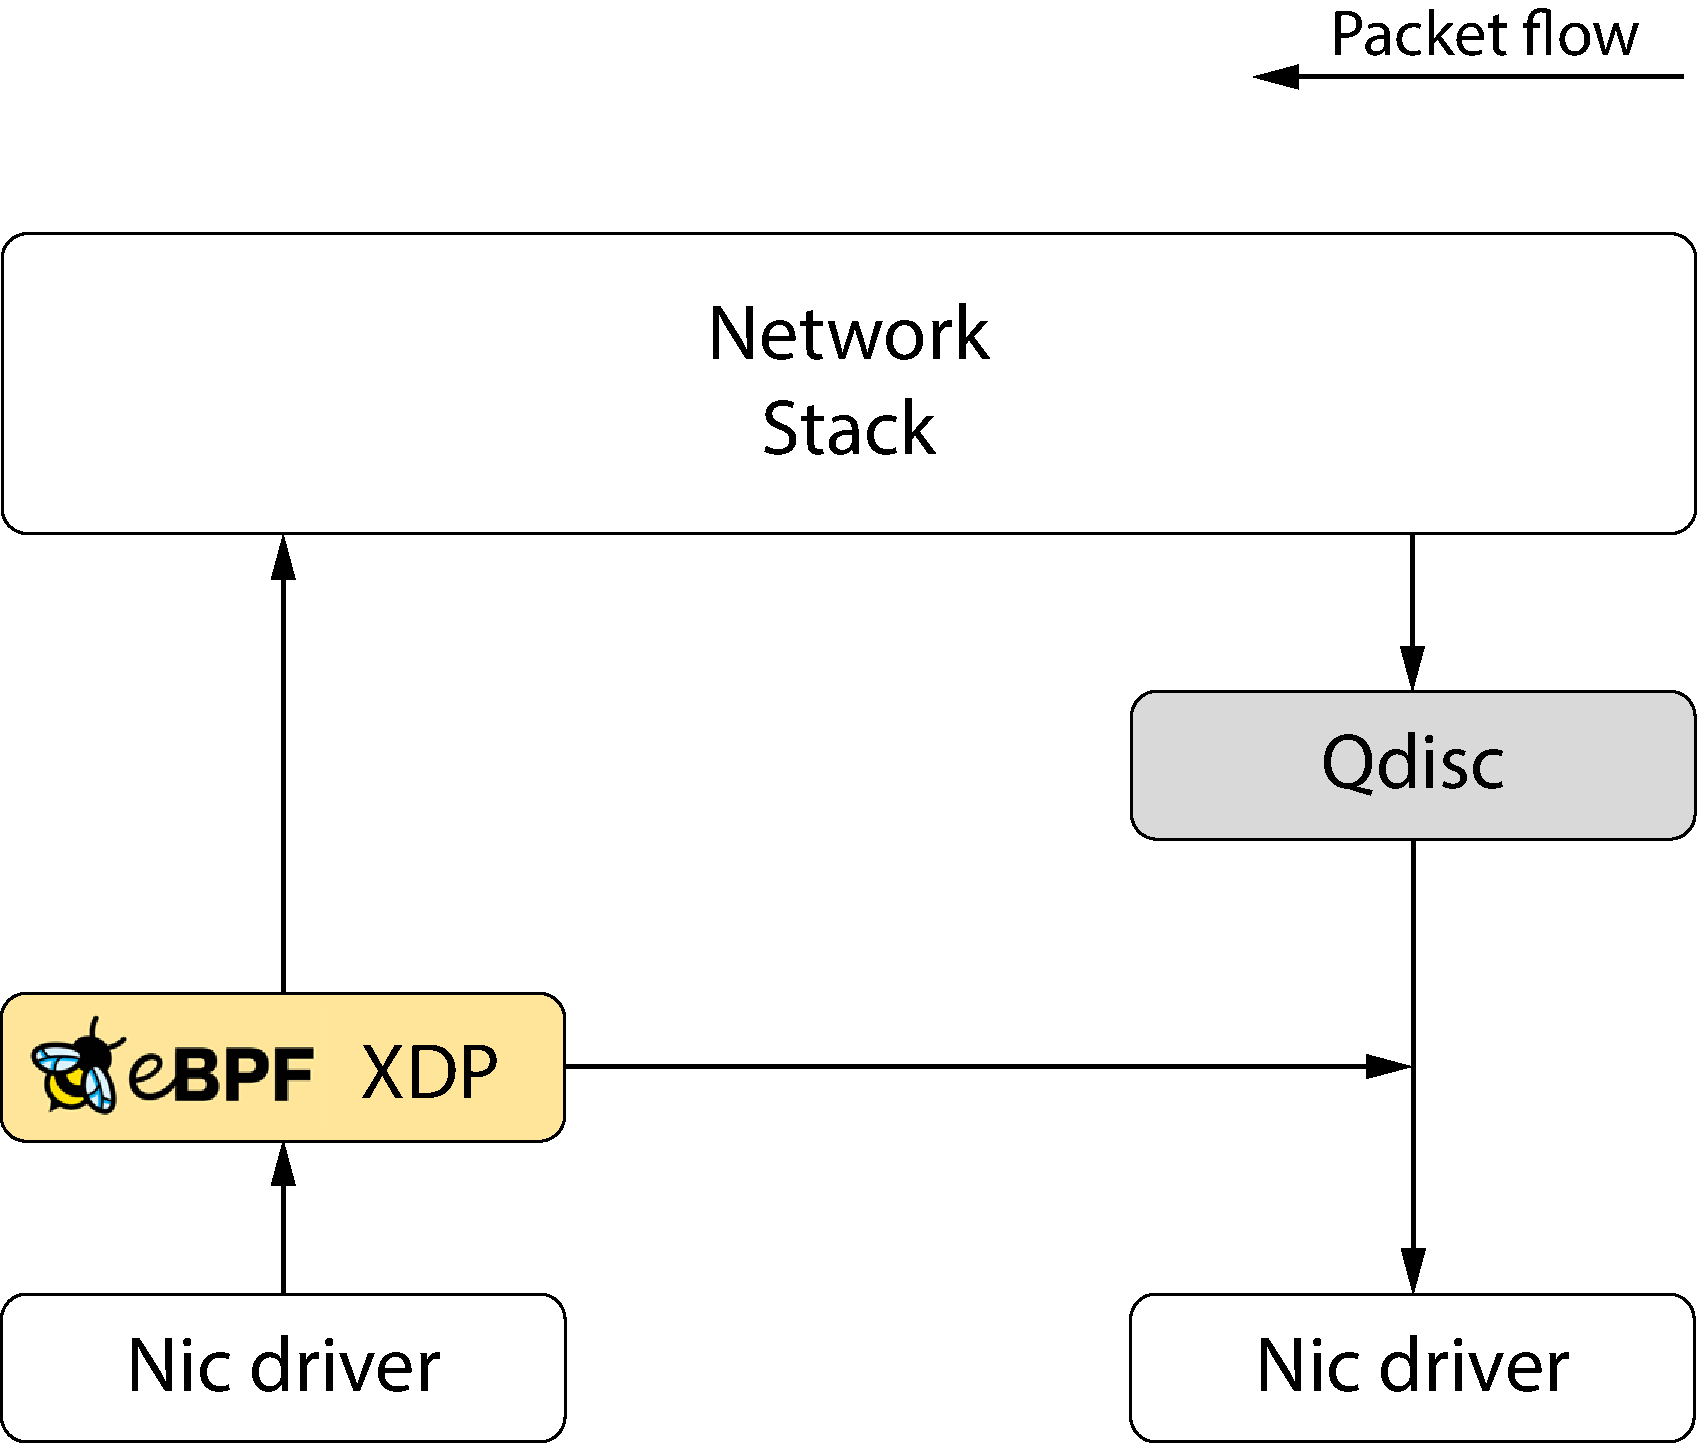
\includegraphics[width=0.6\linewidth]{network-overview.pdf}
  \caption{XDP allows network application programmers to write code that runs on every network packet using the BPF framework. XDP gives the programmer the capability to modify the packet and redirect it using the code's return value. The possible return values are as follows: (i) passing the packet to the kernel's networking stack; (ii) redirecting the packet to another network device; (iii) send the packet directly out on the same device; or (iv) dropping the packet altogether.}
  \label{fig:network_overview}
\end{figure}

The Linux kernel networking stack is highly mature and a flexible piece of software. It contains a hardware abstraction layer, a traffic control layer responsible for routing and firewall rules, and layers responsible for handling the TCP/IP networking layers. Part of the traffic control layer is the queueing discipline layer, or the Qdisc layer for short. This layer gives the Linux kernel flexible packet scheduling capabilities and an interface to create new packet schedulers as loadable kernel modules. However, due to the immense speed increases in modern network devices, the kernel's networking stack has become a bottleneck. This obstacle has prompted network vendors and researchers to create alternative solutions to mitigate this performance bottleneck. One such solution is the Data Plane Development Ki~\cite{dpdk} (DPDK) which entirely bypasses the Linux kernel and communicates directly to the networking hardware. An alternative solution to completely bypassing the Linux kernel, which we describe in \Cref{sec:xdp}, is XDP, which creates a fast data path within the Linux kernel while retaining the kernel and user-space separation. \Cref{fig:network_overview} provides a simplified diagram of the Linux kernel's networking infrastructure depicting the relevant parts related to our work in this paper. The diagram shows how XDP can steer traffic either through the network stack or bypass it altogether.


\section{Programmable Packet Schedulers}

\begin{figure}
  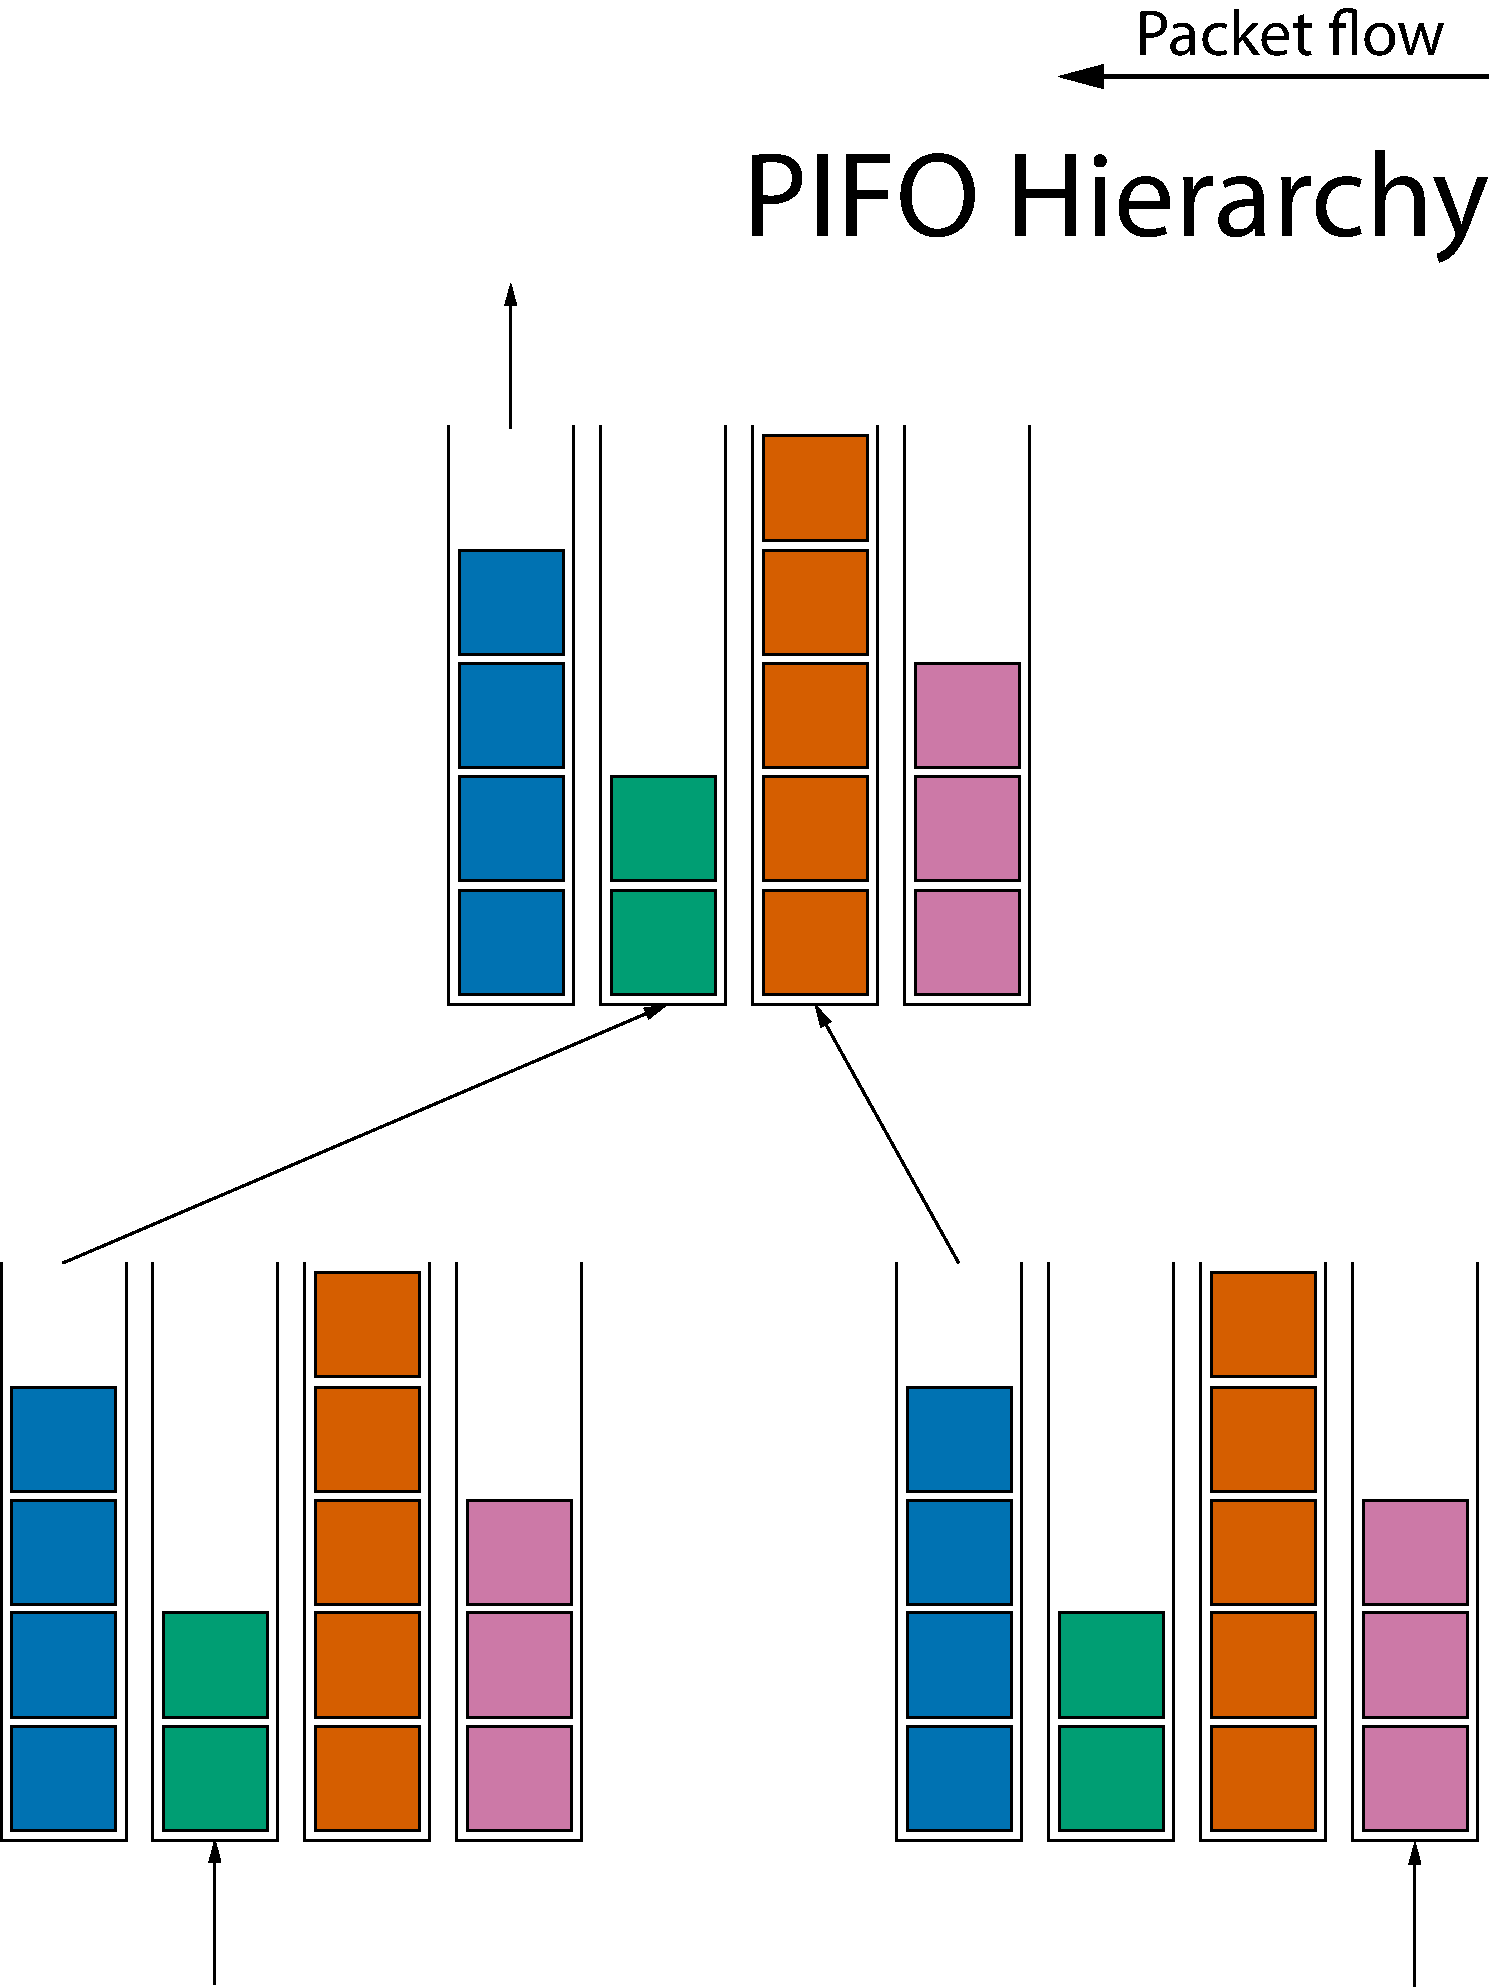
\includegraphics[width=0.5\linewidth]{pifo-hierarchy.pdf}
  \caption{We can implement complex packet scheduling algorithms by forming hierarchies of PIFO and the Eiffel data structures. Some packet schedulers need hierarchies to function. However, we can also use hierarchies to combine different schedulers to handle complex requirements.}
  \label{fig:pifo_hierarchy}
\end{figure}

Traditionally, network equipment and operating systems provide a handful of packet scheduling algorithms. This limited number of schedulers forced companies to tune the parameters of these algorithms to meet their requirements. However, modern networking equipment has started to provide programmable network capabilities, which a network engineer can leverage using specialized programming languages such as P4~\cite{p4} or standard programming languages such as C, such as in the case of traditional operating systems. This new offering allow network designers to create custom logic and custom packet scheduling solutions optimized for their specific unique use case. Therefore, instead of tuning the network to the limitations of the packet scheduling algorithm, they can tune their packet scheduling algorithm directly to their network requirements.

Consequently, the building blocks of a programmable packet scheduling framework need to be straightforward, fast, and easy to understand. Therefore, the essential part of creating a programmable packet scheduling framework is to provide a flexible data structure. Subsequently, this has become an active research area to develop a flexible data structure that programmers can leverage to implement their packet schedulers. However, due to the vast speeds of modern network interfaces, severe time limitations are put on these data structures, which tend to make generic priority queues, such as red-black trees and binary heaps, unsuitable choices.

In this paper, we focus on the two priority queues, PIFO~\cite{Sivaraman2016} and Eiffel~\cite{Saeed2019}, described in \Cref{sec:pifo} and \Cref{sec:eiffel}. Both are simple data structures that share the following qualities: (i) they use an integer-based ranking function to queue packets by their priority and rely on a fixed range of ranks known at initialization time; and (ii) they dequeue according to the scheduled packet order. Furthermore, they both have the flexibility to create complex packet scheduling algorithms by using hierarchies, as seen in \Cref{fig:pifo_hierarchy}. However, Eiffel differs because it can make scheduling decisions on dequeue, while PIFO only makes scheduling decisions on enqueue. This distinction stems from the fact that PIFOs are well suited for hardware and software. However, Eiffel is a software-only data structure and is, therefore, capable of more complex operations, such as flow-based scheduling, which requires scheduling on dequeue.


\subsection{PIFO} \label{sec:pifo}

The Push-In First-Out (PIFO) data structure~\cite{Sivaraman2016} is a priority queue where the programmer can queue packets based on their rank, where each rank is queued in a FIFO order, as shown in \Cref{fig:pifo}. However, the programmer can only dequeue from the head of the PIFO and only order packets on enqueue. Also, the PIFO does not allow reordering the packets within a FIFO. This limitation inhibits the PIFO from implementing some packet scheduling algorithms, such as pFabric~\cite{alizadeh2013pfabric}.

Despite its simplicity, the PIFO data structure is quite versatile and allows the programmer to implement various packet schedulers. From a programmer's perspective, the programmer only needs to decide what order to schedule packets and when to schedule them for non-work conserving algorithms. However, one limitation of the PIFO is that each FIFO, and therefore, each rank, consumes memory. Therefore, the more granular ranks, the more resources the PIFO needs. This limitation limits how large the PIFO can be in hardware and software implementations. A mitigation to this limitation is the SP-PIFO~\cite{Alcoz2020}, which approximates a large PIFO using a smaller PIFO.

\begin{figure}
  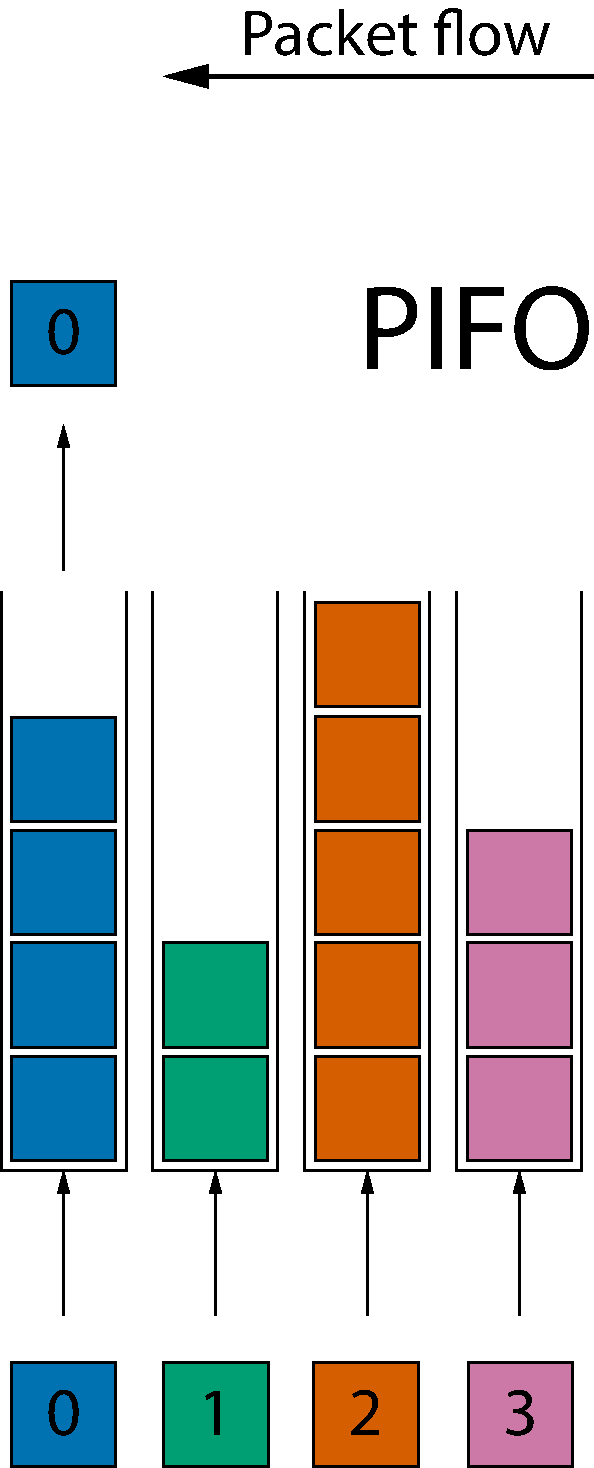
\includegraphics[width=0.25\linewidth]{pifo.pdf}
  \caption{The PIFO data structure is a priority queue where the programmer enqueues packets by rank. However, the dequeue operation can only dequeue packets from the top of the structure. Therefore, the lower priority queues will starve if the highest priority queue keeps getting packets without being emptied.}
  \label{fig:pifo}
\end{figure}


\subsection{Eiffel} \label{sec:eiffel}

The Eiffel~\cite{Saeed2019} data structure is an efficient software implementation of a PIFO with a couple of alterations. First, in Eiffel, the programmer can schedule flows and packets, depending on the algorithm, where each flow is a separate FIFO that contains only the flow's packets. The Eiffel data structure can schedule references to those FIFOs instead of the individual packets. Second, the programmer can do on-dequeue scheduling; this allows the algorithm to virtually rearrange all the packets from the same flow by simply requeueing the reference to that flow back into the Eiffel data structure. These two additions allow the Eiffel data structure to represent more scheduling algorithms than PIFO, such as pFabric~\cite{alizadeh2013pfabric}.

Also, because Eiffel is a software implementation, the Eiffel paper proposes a few software-based optimizations to improve the performance of the Eiffel data structure. One such optimization is to use a bit-field to keep track of queues containing packets and use the CPU's Find-First-Set~\footnote{TODO} instruction to accelerate the lookup in the bit lookup table. The lookup table can be further segmented into a tree-based lookup table when the Eiffel has many ranks.


\section{The BPF framework}

One of the fundamental problems with extending the Linux kernel with specialized code, such as packet schedulers, is writing the extensions as kernel modules. From a security perspective, the modules have access to the entire kernel without limits, making it more prone to programming errors, such as pointer mishandling and infinite loops. The kernel community provides BPF as a safer way of extending the kernel. This framework is an in-kernel runtime environment that allows specialized programs to execute in the kernel safely. To support BPF, kernel programmers add appropriate BPF hooks to the kernel to offer domain-specific extendability to programmers. These hooks allow the programmers to attach BPF code that runs each time these hooks are triggered. The Linux kernel comes with numerous hooks related to networking, tracing, and security, where each hook limits what the BPF code can access and which helper functions it can call.

From a developer perspective, BPF programs are binaries written in the BPF instruction set that can be loaded using the bpf system call into the kernel. This instruction set and runtime are severely limited in functionality. It supports a handful of instructions, and the runtime only has a 512-byte stack. When the kernel loads the binary, it runs it through a BPF verifier that makes sure that all pointers are within bounds, that the program does not call disallowed functions, and that the code cannot run more than a million instructions. After verifying the code, the user-space application can attach the BPF program to the desired hook. However, because each hook provides a different method for attaching BPF programs, it is recommended to use the libbpf~\cite{libbpf} library to load the programs instead.

A salient feature of BPF is that it offers interprocess communication using BPF maps. These maps are key-value stores that act as global variables within the framework and are the primary method to interact with BPF programs. They come in different types, such as arrays and hashmaps, and some of the more advanced maps offer per-CPU storage for additional performance. They provide a common way for different BPF hooks and user-space applications to communicate with each other.


\subsection{XDP} \label{sec:xdp}

Express Data Path (XDP)~\cite{hoiland2018express} is a type of BPF program that is attached directly to the RX path of a network interface to allow the programmer direct manipulation of packets from the network driver. Its primary use cases are high-performance packet processing and the ability to bypass the kernel's network stack by redirecting the packet to different locations, such as back out of the same device, to another device, or dropping the packet entirely. XDP also provides helper functions that allow the programmer to call particular parts of the network stack, such as routing lookups.

\section{A Programmable Packet Scheduling Framework in BPF}

\begin{figure}

  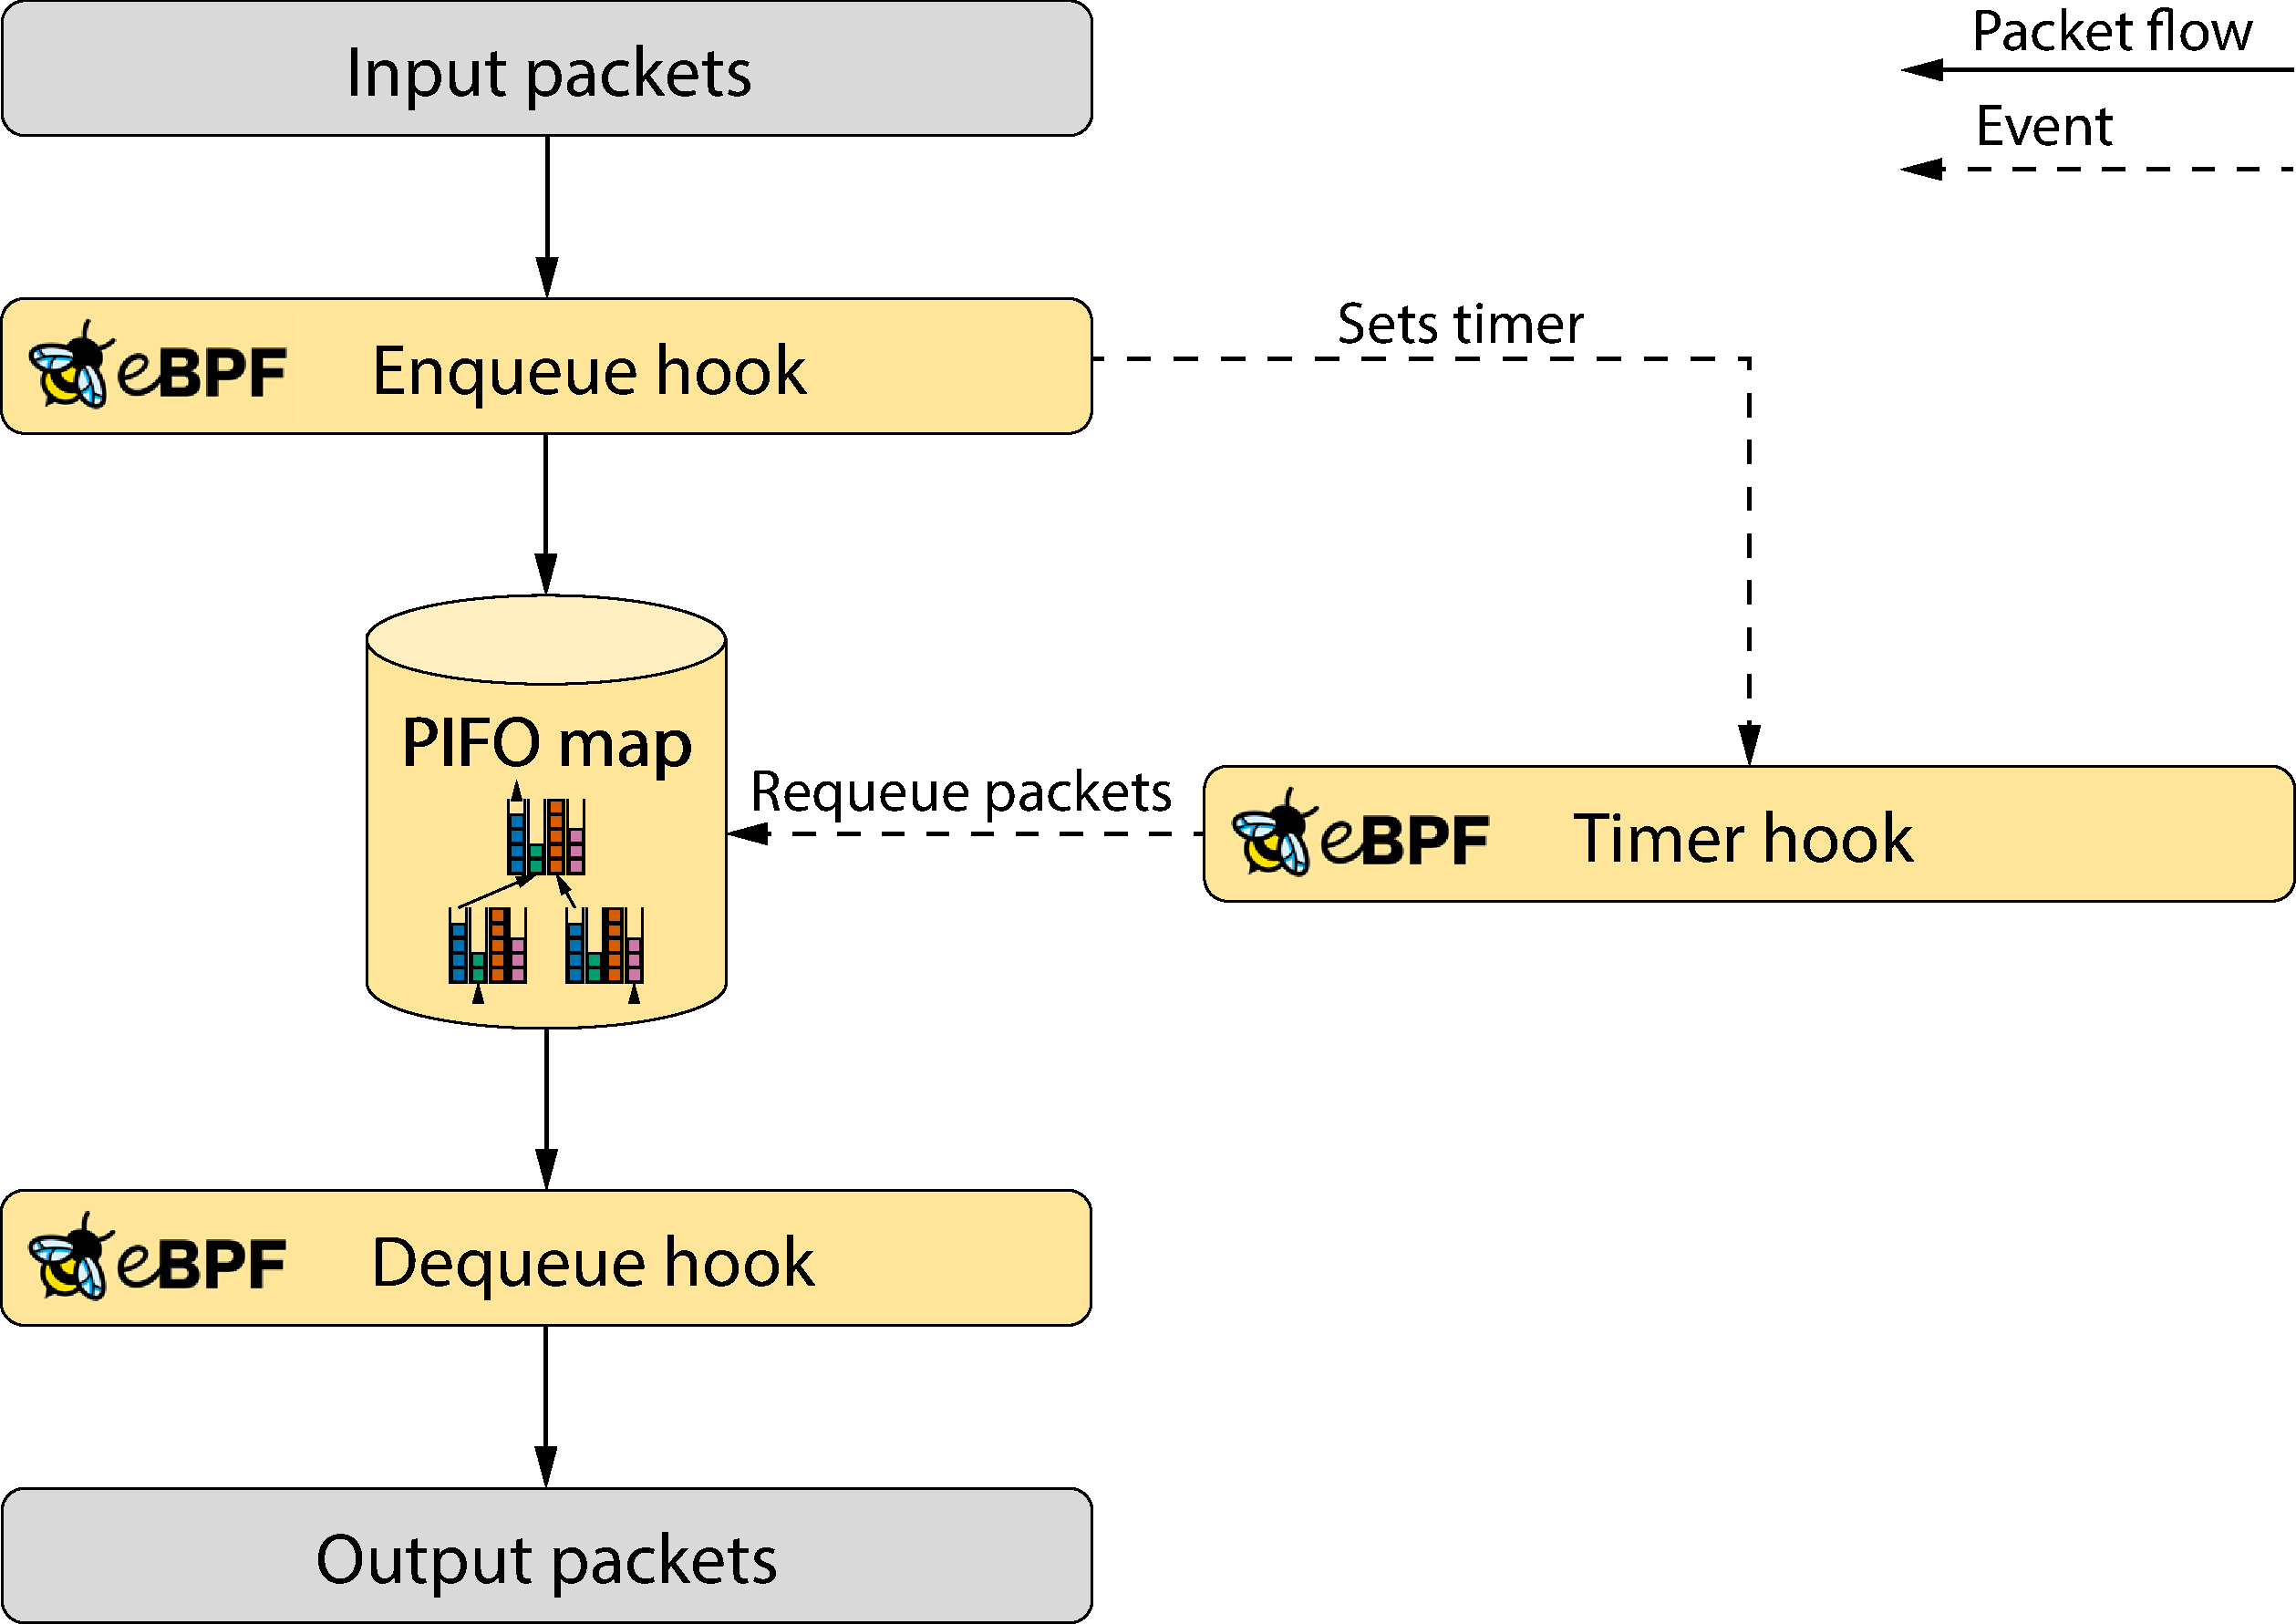
\includegraphics[width=\linewidth]{bpf_pps_flow.pdf}

  \caption{The diagram shows the flow of packets through our proposed BPF-based programmable packet scheduling framework. The framework adds a new dequeue hook to the Linux kernel and a PIFO map. For a fully functional scheduler, the XDP hook must redirect packets to a PIFO, and the dequeue hook must dequeue packets to an interface.}
  \label{fig:bpf_pps_flow}
\end{figure}

While XDP excels at forwarding packets, it does not support packet reordering or scheduling. Our contribution is the extension of XDP to support packet scheduling in BPF using PIFO data structures with Eiffel capabilities. This support includes adding helper functions, a new PIFO BPF map data type, and an extra hook for dequeuing packets from the PIFO data structure. \Cref{fig:bpf_pps_flow} show the design and basic building blocks of our new programmable packet scheduling framework without the specifics of XDP or the Qdisc subsystem.

A more specific description of each component of this new addition is as follows:

\begin{itemize}
        \item PIFO map: This new BPF map implements a PIFO and is the main building block for the programmer to create packet schedulers. The framework provides two variants of this map, a PIFO that can store network packets and a PIFO that can store any data type, including other PIFOs. The second data type gives the programmer a convenient way of creating PIFO hierarchies and scheduling flows instead of packets. These maps come with new helper functions to enqueue and dequeue new packets, and a peek function for the generic PIFO map.
        \item Enqueue hook: This is the standard XDP hook, and in addition to the original capabilities of XDP, it is now capable of redirecting packets to our new PIFO maps.
        \item Dequeue hook: This new hook is responsible for delivering the packet from the packet scheduling algorithm. It can deliver bulking by repeatedly calling the hook to dequeue multiple packets before it transmits them from the interface.
\end{itemize}

Representing the PIFO data structure as a BPF map presents programmers with a familiar map interface that they have come accustomed to in BPF. From a programmer's perspective, the BPF hooks reference the queues like any other map type. The enqueue hook decides which queue to direct the packet to by a map reference. Similarly, the dequeue hook picks which queue map to dequeue from and returns a reference to the dequeued packet to the kernel for transmission.


\section{Future Work}

Our current implementation gives XDP the capability to schedule packets; however, it is still missing the capability to implement pacing. We are working on adding pacing to our packet scheduling framework by using the newly added BPF timers, which will allow the programmer to redirect packets to PIFOs triggered using timers set in the XDP hook. These timers allow the PIFO dequeue hooks to enqueue the packets into other PIFOs that dequeue into live interfaces or other timer-triggered PIFOs—giving our framework pacing capabilities.

While we believe that scheduling in XDP will benefit today's high-speed environments, a few outstanding research questions remain. On the Linux kernel side, we assume that the Eiffel PIFO extensions outperform the kernel's red-black trees due to the PIFO's complexity of $\mathcal{O}(1)$, compared to the red-black tree's $\mathcal{O}(\log_{2}{}n)$. However, it remains an open research question if this is the case in practice with the short queue lengths our schedulers need. Another missing benchmark is comparing our framework against the kernel's Qdisc layer and how much performance is gained.


\section{Conclusion}

Current networking technologies have reached speeds that have pushed the industry and researchers to explore alternative solutions to remove bottlenecks in the networking stack. One of these solutions is XDP, which allows programmers to bypass the kernel. However, XDP did not have a way to rearrange or schedule packets. In our work, we have created a packet scheduling framework for XDP, which allows the programmer to write domain-specific packet schedulers while retaining all the benefits of XDP.


\bibliographystyle{ACM-Reference-Format}
\bibliography{references}


\end{document}
\endinput
